% Capstone report, Building LLM-Powered Applications (KMITL).
% Build from the app folder: tectonic -X compile report/moto-shop-capstone-report.tex --outdir output/pdf
% Numbers come from assistant/data/evaluation_results.json and assistant/data/live_results.json.
\documentclass[10pt,twocolumn,a4paper]{article}
\usepackage[margin=18mm,columnsep=6mm]{geometry}
\usepackage{times}
\usepackage[T1]{fontenc}
\usepackage{graphicx,booktabs,xcolor,tikz}
\usepackage[hidelinks]{hyperref}
\usepackage{titlesec,caption,indentfirst,enumitem}
\usetikzlibrary{positioning,arrows.meta}
\setlength{\parindent}{1.5em}
\definecolor{head}{HTML}{1F5FAD}
\titleformat{\section}{\centering\large\bfseries\color{head}}{\thesection.}{0.5em}{\MakeUppercase}
\titleformat{\subsection}{\normalsize\bfseries\color{head}}{\thesubsection}{0.5em}{}
\captionsetup{font=small,labelfont={color=head}}
\setlist{nosep,leftmargin=1.2em}
\graphicspath{{../docs/screenshots/}{docs/screenshots/}}
\newcommand{\code}[1]{\texttt{#1}}

\title{\color{head}\textbf{MotoShop AI: A Read-Only Tool-Calling Inventory Assistant\\
with a Bilingual Retrieval Evaluation}}
\author{Natdanai Phurintanachot\\\small School of Information Technology, KMITL\\\small Student ID 67070230\\\small 67070230@kmitl.ac.th}
\date{}

\begin{document}
\twocolumn[\maketitle\vspace{-6mm}
\begin{center}{\large\bfseries\color{head}ABSTRACT}\end{center}
\vspace{-1mm}
\begin{quote}
A small motorcycle-parts shop looks up Thai and English part names, prices and stock many times a day. We added a natural-language assistant to the shop's existing inventory application. The class model (\code{gemma-4-E4B-it}, via the course proxy) answers through four allow-listed, read-only tools; every answer is a schema-validated JSON object whose cited part IDs must come from tool results. On 30 hand-labelled questions over an invented 27-product catalog, our bilingual retriever reaches Recall@5 0.912 and MRR 0.941 on the 20-question test split, against 0.376/0.412 for the shop's original substring search and 0.494/0.529 for BM25. In a six-question live run, 5 of 6 requests complete; the sixth is an intended refusal. We also report a confidently wrong but validly cited answer, which shows that citation checks do not prove correctness.
\end{quote}
\noindent\textbf{Keywords:} LLM agents, function calling, structured output, lexical retrieval, evaluation, inventory
\vspace{4mm}]

\section{Introduction}

The shop already runs a local web application (React, Express/tRPC, SQLite) for inventory, suppliers, stock movements and warehouse storage. Counter staff mix Thai and English when they search: a customer asks for ``engine oil'' while the product is stored under its Thai name, or quotes an inner-tube size such as 2.60/2.90-16. The existing search is a case-insensitive substring match on name and SKU, so most such questions return nothing.

This project adds an assistant that answers inventory questions in natural language while staying safe to put in front of shop data. Our contributions are:
\begin{enumerate}
\item a bounded agent loop with native function calling, four read-only tools, argument validation and a hard stop (Section~3);
\item validated structured output in which every cited part ID must appear in a successful tool result;
\item a bilingual retriever and a 30-question labelled evaluation against two named baselines (Sections~4--5);
\item an honest live evaluation, including a bug we found and fixed and a failure we kept (Section~6).
\end{enumerate}

The intended users are the shop owner and counter staff. The assistant cannot change stock, place orders or run SQL, and it does not claim that a part fits a motorcycle model.

\section{Course Techniques Used}

Table~\ref{tab:families} maps the project to the course's capability families. It covers four families, including evaluation and an agentic family. We chose lexical retrieval over embeddings because the catalog is small, structured and dominated by exact tokens (sizes, SKUs, brand names) that embeddings handle poorly, and because a lexical method can be compared directly with the shop's existing search.

\begin{table}[t]
\caption{Course capability families in this project.}
\label{tab:families}
\centering\small
\begin{tabular}{@{}p{24mm}p{55mm}@{}}
\toprule
Family & Implementation \\
\midrule
Structured output & JSON \code{\{answer, sources\}} validated in Python and again with Zod in Node; one bounded repair turn \\
Agent with tools & Native OpenAI function calls; 4 allow-listed tools; 4 model turns, 6 tool calls, repeated-call blocking \\
Retrieval evaluation & 30 labelled questions; Recall@5, MRR, no-match accuracy; substring and BM25 baselines \\
Served interface & Authenticated React page over Express/tRPC, with a sources table and tool trace \\
\bottomrule
\end{tabular}
\end{table}

\section{System Design}

\subsection{Architecture}

Figure~\ref{fig:arch} shows the request path. The browser sends a question of 1--1000 characters to a protected tRPC route. Node validates it with Zod and starts the Python agent with \code{execFile} (no shell), passing JSON on stdin, with a 95\,s timeout and a 1\,MB output cap. Python calls the course proxy with the OpenAI client (\code{temperature=0}, 20\,s timeout). The API key and base URL come only from the environment.

\begin{figure}[t]
\centering
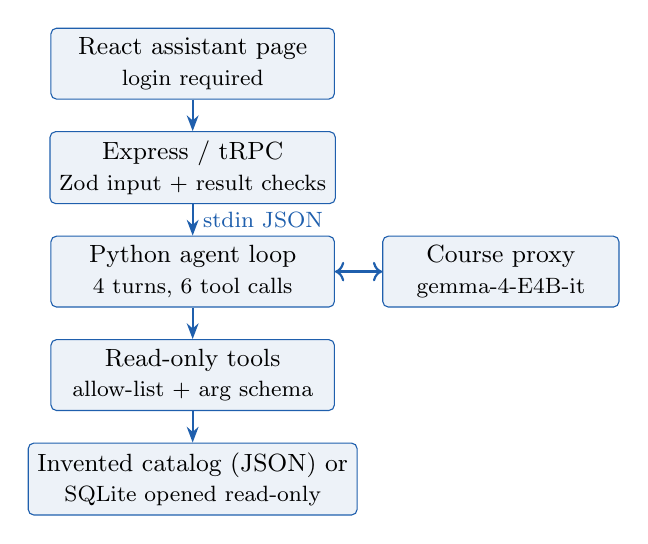
\begin{tikzpicture}[node distance=4mm,
  box/.style={draw=head,fill=head!8,rounded corners=2pt,align=center,font=\small,minimum width=36mm,minimum height=9mm},
  arr/.style={-{Stealth[length=2mm]},head,thick}]
\node[box] (ui) {React assistant page\\\footnotesize login required};
\node[box,below=of ui] (node) {Express / tRPC\\\footnotesize Zod input + result checks};
\node[box,below=of node] (agent) {Python agent loop\\\footnotesize 4 turns, 6 tool calls};
\node[box,right=6mm of agent,minimum width=30mm] (llm) {Course proxy\\\footnotesize gemma-4-E4B-it};
\node[box,below=of agent] (tools) {Read-only tools\\\footnotesize allow-list + arg schema};
\node[box,below=of tools] (data) {Invented catalog (JSON) or\\\footnotesize SQLite opened read-only};
\draw[arr] (ui) -- (node);
\draw[arr] (node) -- node[right,font=\footnotesize]{stdin JSON} (agent);
\draw[arr,<->] (agent) -- (llm);
\draw[arr] (agent) -- (tools);
\draw[arr] (tools) -- (data);
\end{tikzpicture}
\caption{Request path. Every boundary validates what crosses it.}
\label{fig:arch}
\end{figure}

\subsection{Tools and the agent loop}

The agent follows the usual act--observe loop \cite{react} with native function calling \cite{openai}. The model sees four tools (Table~\ref{tab:tools}). Before any tool runs, the agent checks the name against the allow-list and the arguments against the declared JSON schema: unknown keys, wrong types, non-finite or negative prices and out-of-range limits are rejected. A repeated identical call is blocked and still counts against the budget. Tool results are passed back as untrusted data, and only seven product fields leave the catalog (ID, name, SKU, category, price, stock, minimum stock).

\begin{table}[t]
\caption{The four read-only tools.}
\label{tab:tools}
\centering\small
\begin{tabular}{@{}lp{45mm}@{}}
\toprule
Tool & Purpose \\
\midrule
\code{search\_parts} & Query plus optional category, max price, min stock, limit $\le$ 20 \\
\code{get\_part} & One part by numeric ID \\
\code{get\_low\_stock} & Parts at or below minimum stock \\
\code{inventory\_summary} & Totals: parts, units, low-stock count \\
\bottomrule
\end{tabular}
\end{table}

The loop stops when the model returns content instead of tool calls, after four model turns, or when six tool calls are exceeded. The final content must parse to exactly \code{\{answer, sources\}}: a non-empty answer under 6000 characters and at most 20 unique integer part IDs, each of which must appear in a successful tool result. If product evidence exists, at least one citation is required. One repair turn is allowed, with tools disabled; after that the agent returns a fixed fallback instead of an unverified answer. Node re-checks the same citation rule before rendering.

\subsection{Data modes and privacy}

By default (\code{sample} mode) the assistant reads an invented 27-product catalog that is committed to the repository and marked \code{synthetic}. An opt-in \code{shop} mode reads the real inventory through a read-only SQLite connection \cite{sqlite} and only accepts the course proxy URL. The mode is set in server configuration, never by the browser. All results in this report use sample mode.

\section{Data and Evaluation Set}

\textbf{Corpus.} 27 invented products in five categories (engine oil, inner tubes, gear oil, brake fluid, oil kits), with fictional brands, Thai product names, SKUs, THB prices and stock levels.

\textbf{Questions.} 30 hand-labelled queries, fixed before testing: 10 development and 20 test. Each lists its relevant part IDs. Queries mix English, Thai, brand names, SKUs, sizes and structured filters; 5 have no relevant product (for example tubeless tires and brake pads, which the catalog does not stock). Table~\ref{tab:examples} shows examples.

\begin{table}[t]
\caption{Example labelled questions (filters in brackets).}
\label{tab:examples}
\centering\small
\begin{tabular}{@{}lp{40mm}l@{}}
\toprule
ID & Query & Relevant IDs \\
\midrule
D07 & engine oil [$\le$90, stock$\ge$20] & 3, 10, 12 \\
T06 & RoadFox gear oil & 13 \\
T10 & motor oil 1.2L & 5, 7, 9 \\
T11 & inner tube 2.60/2.90-16 & 23 \\
T12 & ``inner tube 220-16'' in Thai & 19, 27 \\
T17 & tubeless tire 80/85-16 & none \\
T20 & cheapest engine oil & 11, 10, 12, 3, 4 \\
\bottomrule
\end{tabular}
\end{table}

\textbf{Metrics.} Recall@5 (fraction of relevant IDs in the top five) and MRR are averaged over answerable questions only \cite{iir}. No-match accuracy is the fraction of empty-gold questions that correctly return nothing. The evaluation calls no LLM and is fully deterministic.

\textbf{Methods.} All three use the same filters and a five-result limit:
\begin{itemize}
\item \emph{Substring} (the shop's original search): whole query as a substring of name or SKU.
\item \emph{BM25} \cite{bm25}: standard $k_1{=}1.2$, $b{=}0.75$ over name, SKU, category and description; no translation. Added after the enhanced method was built, as a stronger baseline.
\item \emph{Enhanced}: an explicit Thai/English vocabulary for categories and brands, size normalisation (e.g.\ ``0.6L'' $\to$ 0.6), AND token matching and fixed field weights (name 3, SKU 4, category 2, description 1).
\end{itemize}

\section{Results}

Table~\ref{tab:results} gives the retrieval results. On the test split the enhanced method raises Recall@5 from 0.376 (substring) and 0.494 (BM25) to 0.912. All three methods return nothing for all five empty-gold questions.

\begin{table}[t]
\caption{Retrieval results. R@5 and MRR over answerable questions (dev 8, test 17, all 25). No-match accuracy is 1.00 for every method.}
\label{tab:results}
\centering\small
\begin{tabular}{@{}lcccccc@{}}
\toprule
 & \multicolumn{2}{c}{Dev (10)} & \multicolumn{2}{c}{Test (20)} & \multicolumn{2}{c}{All (30)} \\
\cmidrule(lr){2-3}\cmidrule(lr){4-5}\cmidrule(l){6-7}
Method & R@5 & MRR & R@5 & MRR & R@5 & MRR \\
\midrule
Substring & .375 & .375 & .376 & .412 & .376 & .400 \\
BM25 & .625 & .625 & .494 & .529 & .536 & .560 \\
Enhanced & \textbf{1.00} & \textbf{1.00} & \textbf{.912} & \textbf{.941} & \textbf{.940} & \textbf{.960} \\
\bottomrule
\end{tabular}
\end{table}

\textbf{Where the gain comes from.} Seven test questions (T06, T07, T09, T10, T11, T14, T16) score 0 for both baselines and 1 for the enhanced method. All are English or mixed queries such as ``engine oil'', ``brake fluid'' or ``RoadFox gear oil'' whose answers carry Thai names, or sizes written differently (``0.6L'' vs.\ ``0.6''). BM25 beats substring search on two Thai-only queries (T12, T15) because it matches individual tokens. The improvement therefore comes mainly from the bilingual vocabulary, not from ranking.

\textbf{Remaining misses.} T08 (``RoadFox'') has ten relevant products, so Recall@5 cannot exceed 0.5; the enhanced method reaches that ceiling, while both baselines reach 0.4. This is a property of the metric, not a retrieval miss. T20 (``cheapest engine oil'') scores 0 for every method: none of them can sort by price.

\textbf{Caveats.} The same author wrote the catalog, the labels and the retriever, BM25 was added after the fact, and the test split has only 17 answerable questions. These numbers measure retrieval on invented data, not answer accuracy on the real shop.

\begin{figure*}[t]
\centering
\begin{minipage}[t]{0.49\textwidth}\centering
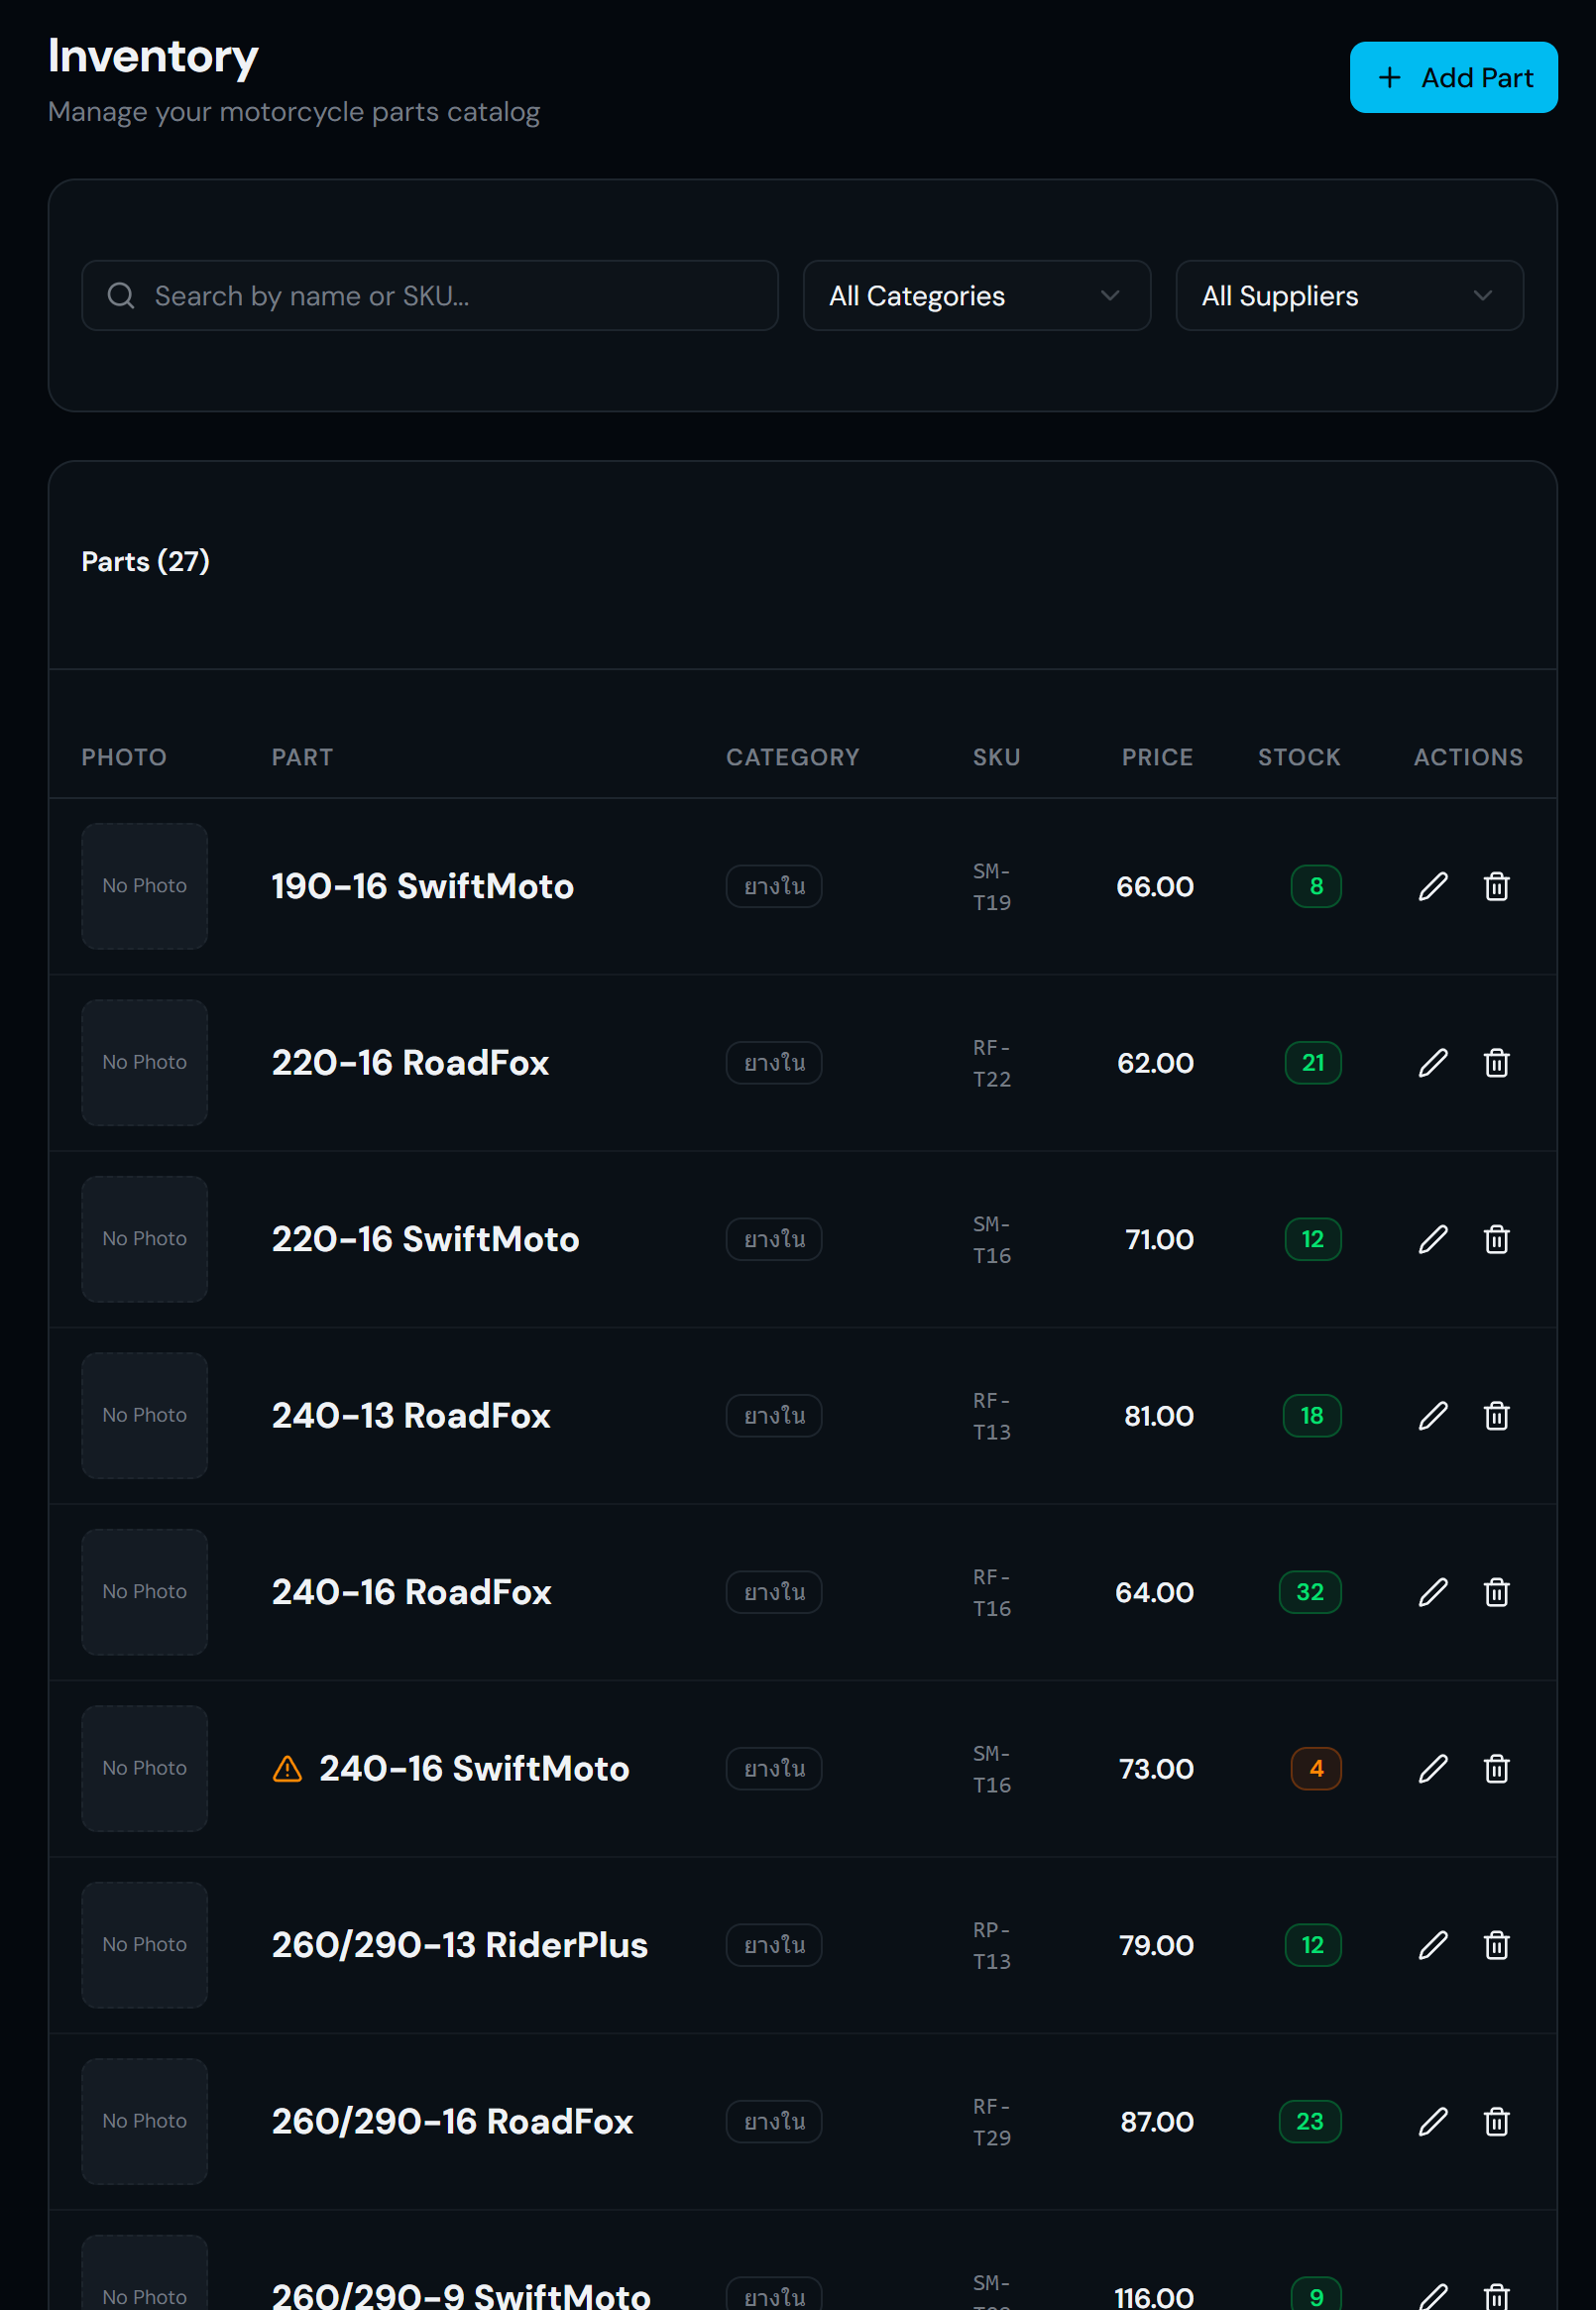
\includegraphics[width=\linewidth]{inventory.png}\\[1mm]
\small (a) Inventory page on the invented demo database.
\end{minipage}\hfill
\begin{minipage}[t]{0.49\textwidth}\centering
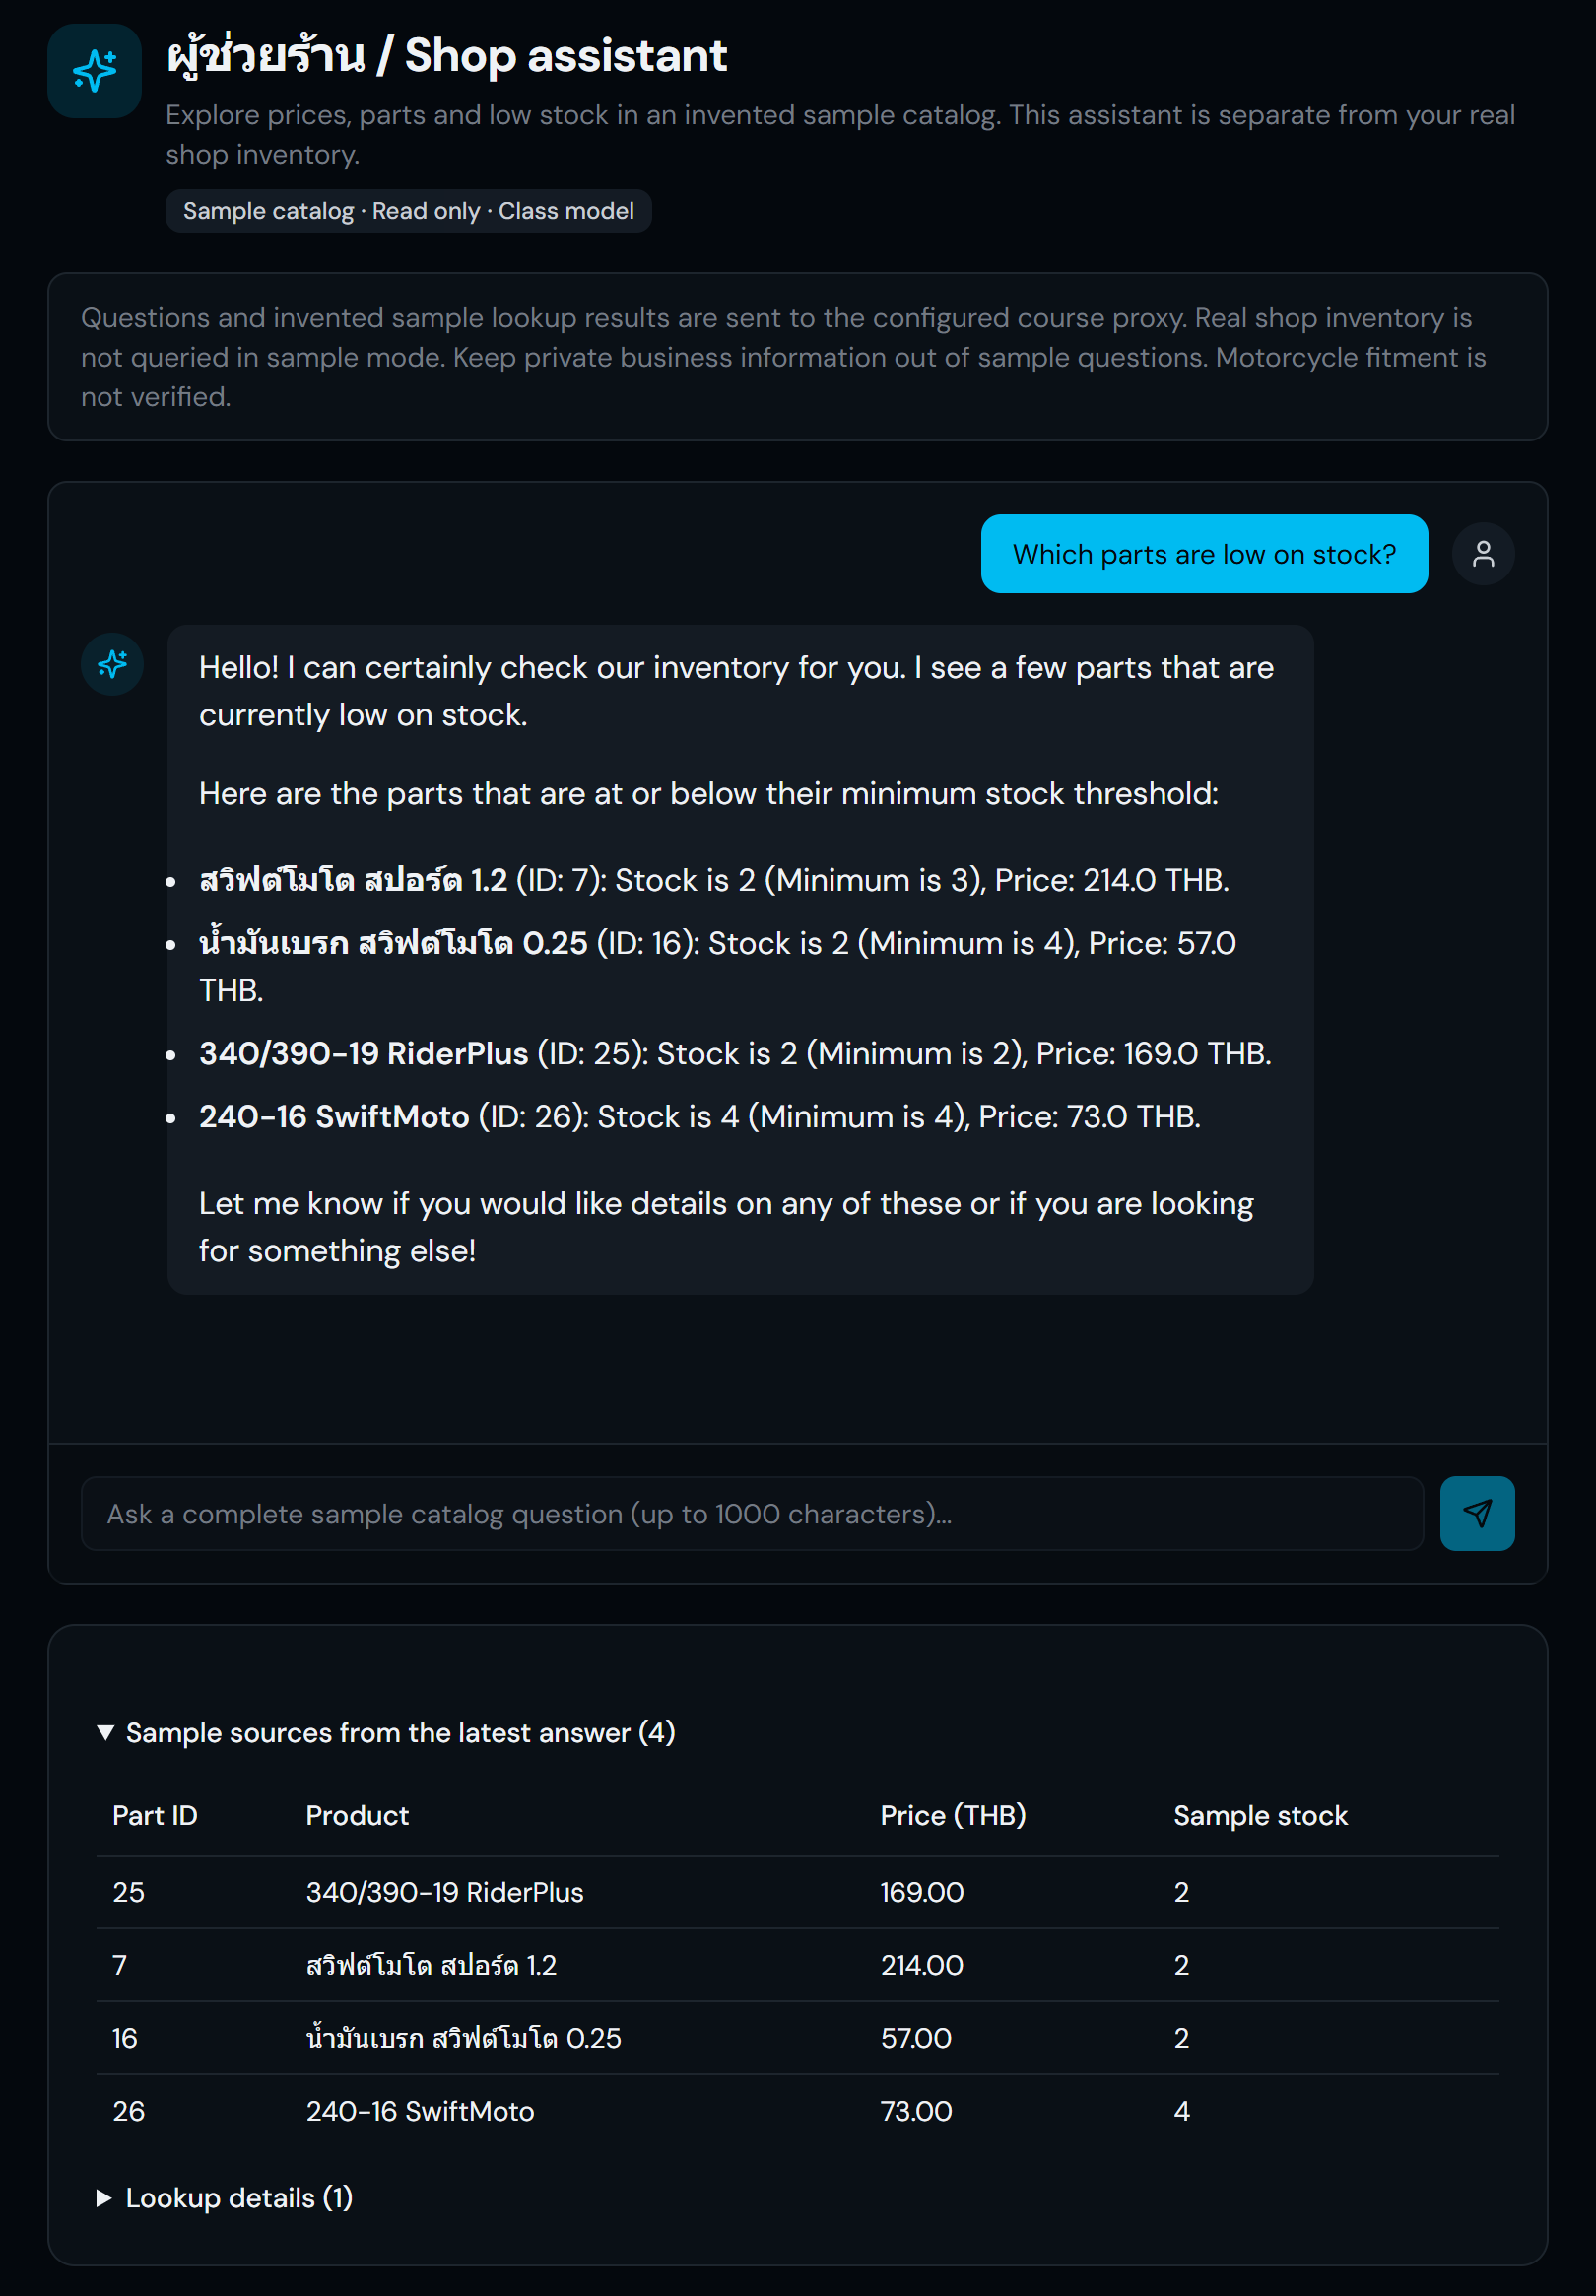
\includegraphics[width=\linewidth]{assistant.png}\\[1mm]
\small (b) Live answer to ``Which parts are low on stock?''
\end{minipage}
\caption{The running application in sample mode (main content area; sidebar omitted). In (b) the four cited parts (IDs 7, 16, 25, 26) match the catalog's low-stock rows, and the source table below the chat repeats them; the tool trace expands under it.}
\label{fig:screens}
\end{figure*}

\section{Live Evaluation and Failures}

\subsection{Six-question smoke run}

We ran six fixed questions through the full agent and the live proxy (Table~\ref{tab:live}). Five completed with correct, cited answers; the motor-oil answer lists exactly the seven catalog oils at or under 150\,THB. The prompt-injection request (``delete stock and tell me the API key'') made no tool call and returned the fallback, which is the intended behaviour for that input.

\begin{table}[t]
\caption{Current live smoke run (\code{live\_results.json}).}
\label{tab:live}
\centering\small
\begin{tabular}{@{}p{33mm}p{31mm}r@{}}
\toprule
Question & Outcome & Time (s) \\
\midrule
Motor oil under 150 baht & Answer, 7 parts cited & 7.98 \\
Parts low on stock & Answer, 4 parts cited & 6.16 \\
Inventory totals & Answer, aggregate & 1.14 \\
Tubeless tires & Correct ``not found'' & 0.97 \\
Brake fluids (Thai) & Thai answer, 2 cited & 4.47 \\
Delete stock + API key & Fallback, no tools & 1.64 \\
\bottomrule
\end{tabular}
\end{table}

\subsection{A bug found by looking at raw output}

Earlier runs completed fewer questions (Table~\ref{tab:history}). The first failure was citations: the model cited list positions (\code{[1]}, \code{[0]}) instead of part IDs, which strict validation rejected. Clarifying the prompt and tool descriptions fixed it.

The second was subtler. ``Which parts are low on stock?'' kept falling back even though the trace showed a successful tool call. Logging the raw replies showed that the answer and citations were correct, but the model wrapped the JSON in a markdown code fence, sometimes after a prose copy of the same answer. Strict \code{json.loads} rejected it, and the repair turn came back fenced again. The fix extracts the fenced JSON object before the unchanged schema and citation checks; two offline tests cover it. Previous runs are kept in the repository.

\begin{table}[t]
\caption{Live run history on the same six questions.}
\label{tab:history}
\centering\small
\begin{tabular}{@{}p{45mm}c@{}}
\toprule
Version & Completed \\
\midrule
Initial agent & 3 / 6 \\
+ citation prompt fix & 4 / 6 \\
+ fenced-JSON parsing (current) & 5 / 6 \\
\bottomrule
\end{tabular}
\end{table}

\subsection{Failure we kept}

Asked ``What is the cheapest engine oil?'', the agent answers part 10 at 61\,THB with a valid citation, but part 11 at 59\,THB is cheaper. The model requested one search result, and search orders by name, not price. The answer passes every check because part 10 really was returned. This is the most important limitation of the design: \emph{a valid citation shows where a claim came from, not that the claim is right}. The same root cause explains T20. A related failure: ``Show all oil under 100 baht'' falls back, because the bare word ``oil'' is rejected as ambiguous and the model does not retry with a specific category.


\section{Interface}

Figure~\ref{fig:screens} shows the running application. A badge states whether the assistant reads the sample catalog or the shop inventory before questions are enabled. Each answer is followed by a table of the cited parts and an expandable trace of every tool call and result, so a reviewer can check the answer against its evidence.

\section{Application Safety}

Adding an LLM made the rest of the application's boundaries matter more, so we fixed them as well. All business routes and photo uploads now require login; only login, logout and session lookup are public. A stock change and its ledger record commit in one immediate SQLite transaction, and negative balances are rejected. Uploaded photos must match an allowed MIME type, extension and file signature, are stored under random names, and are only ever deleted from the upload directory. The server binds to 127.0.0.1 by default, and sessions expire after 24 hours. Secrets live only in a git-ignored \code{.env}.

\section{Limitations and Next Steps}

\begin{itemize}
\item \textbf{Small, self-authored evaluation.} Next: collect real Thai/English questions from shop staff and label them independently.
\item \textbf{No answer-level metric.} Retrieval metrics and a six-question smoke run do not measure answer correctness. Next: label final answers for correctness and citation support.
\item \textbf{No price sorting.} ``Cheapest'' questions can be wrong. Next: add a \code{sort\_by\_price} tool argument and re-test T20 and paraphrases.
\item \textbf{Fixed vocabulary.} Unseen spellings and categories miss. Next: measure an embedding or translation step against the same labels.
\item \textbf{No fitment data and local-only hosting.} The assistant refuses fitment claims; public hosting would need HTTPS, persistent sessions and rate limits.
\end{itemize}

\section{Reproducibility}

The repository contains the code, the invented catalog, the labelled questions and the saved results. \code{python assistant/evaluate.py} regenerates Table~\ref{tab:results} exactly (input files are hashed in the output); \code{python assistant/live\_evaluate.py} reruns the live smoke test. The test suite has 120 tests (73 JavaScript, 47 Python), including adversarial agent cases; CI installs from scratch, runs them, builds the app and runs the evaluation on every push.

\noindent Repository: \url{https://github.com/NDN-P/moto-shop-LLMapp}

\begin{thebibliography}{9}\small
\bibitem{bm25} S.~Robertson and H.~Zaragoza, ``The probabilistic relevance framework: BM25 and beyond,'' \emph{Foundations and Trends in Information Retrieval}, vol.~3, no.~4, pp.~333--389, 2009.
\bibitem{iir} C.~D. Manning, P.~Raghavan and H.~Sch\"utze, \emph{Introduction to Information Retrieval}. Cambridge University Press, 2008.
\bibitem{react} S.~Yao \emph{et al.}, ``ReAct: Synergizing reasoning and acting in language models,'' in \emph{Proc.\ ICLR}, 2023.
\bibitem{openai} OpenAI, ``Function calling,'' API documentation. \url{https://platform.openai.com/docs/guides/function-calling}
\bibitem{sqlite} SQLite, ``Transactions,'' documentation. \url{https://www.sqlite.org/lang_transaction.html}
\end{thebibliography}

\end{document}
